\chapter{Intégrales, Primitives}
`
\textbf{Pré-requis: } Fonctions continues sur un intervalle, dérivée, 

\section{Primitives: vocabulaire, définitions et propriétés}
\begin{mydef}
  Soit f une fonction continue sur un intervalle I. Une fonction F,
  définie sur I, est une \textbf{primitive de la fonction f} sur I si
  F est dérivable et pour tout x de l'intervalle I on a $F'(x) = f$
\end{mydef}

\exemple{}: On considère la fonction f définie sur $\R$ par $f(x) = 6$
pour tout x de $\R$. La fonction F définie sur $\R$ par $F(x) = 6x$
est une primitive de f. En effet, F est dérivable sur $\R$ et $F'(x) =
6 = f(x)$ pour tout x de $\R$. Si on définit maintenant la fonction G
définie sur $\R$ par $G(x) = 6x + 4$, alors G est aussi une primitive
de f sur $\R$. En effet, G est dérivable sur $\R$ et on a $G'(x) = 6 =
f(x)$.

Cet exemple amène donc à la proposition suivante:

\begin{prop}
  Si une fonction admet une primitive sur un
  intervalle I alors elle en admet une infinité.
\end{prop}

\begin{Proof}
  On note F la primitive de f sur I qui existe par hypothèse. On pose
  G la fonction définie sur I par $G(x) = F(x) + k $ où k est une
  constante de $\R$. Alors G est aussi une primitive de f sur I. En
  effet, G est dérivable, car F est dérivable, et $G'(x) = F'(x) =
  f(x)$. 
\end{Proof}

\begin{Rem}
  Toute primitive F de la fonction f est définie à une constante
  près. L'ensemble des primitives G de la fonction f est définie par
  $G(x) = F(x) + k$ où k est un réel. 
\end{Rem}

\begin{Proof}
  On a déjà montré que si f admettait une primitive F sur I alors
  l'ensemble des fonctions G définies sur I par $G(x) = F(x) + k$
  définit un ensemble de primitive de f sur I.

  Il reste donc à montrer que si f admet une deuxième primitive G sur
  I alors G est forcément de la forme $F(x) + k$ où k est un réel.
  Soit G une primitive de f sur I. On note $h:x \mapsto G(x) -
  F(x)$. On a $h'(x) = G'(x) - F'(x) = f(x) - f(x) = 0$. Ainsi pour
  tout x de \textbf{l'intervalle} I $h'(x) = 0$ donc h est constante
  sur I. Ainsi, il existe un réel k, tel que $h(x) = k$ pour tout x de
  $I$. Finalement, on arrive à $G(x) - F(x) = k $ pour tout x de $I$
  et donc $G(x) = F(x) +k$ pour tout x de l'intervalle I.
\end{Proof}

\begin{theo}[Primitives et condition d'égalité en un point]
  Soit f une fonction continue sur un intervalle I. Soient $x_0 \in I$
  et $y_0 \in \R$. Il existe une \textbf{unique} primitive $F_0$ de f sur I
  qui est telle que $F_0(x_0) = y_0$. 
\end{theo}

\begin{Proof}
  \textbf{Existence}:

  On a vu que toutes les primitives de la fonction f sur l'intervalle
  I sont de la forme $x \mapsto F(x) + k$ où F est une primitive de f
  sur I et k un réel. Pour que $F_0$ vérifie la condition imposée on
  doit avoir: $F_0(x_0) = y_0$ ou encore $F_0(x_0) = F(x_0) + k =
  y_0$. En posant $k = y_0 - F(x_0)$ on a bien:
  \[
    F_0(x_0) = F(x_0) + y_0 - F(x_0) = y_0
  \]
  \newline
  \textbf{Unicité: }

  Supposons qu'il existe $F_1$ et $F_2$ définies sur I tels que:
  \begin{enumerate}[label = (\arabic*),leftmargin=2cm]
  \item $F_1$ et $F_2$ sont des primitives de f sur I
  \item $F_1(x_0) = F_2(x_0) = y_0$
  \end{enumerate}
  et montrons que $F_1 = F_2$ sur l'intervalle I tout entier.

  On note h la fonction définie sur I par $h: x \mapsto F_1(x) -
  F_2(x)$. On a $h'(x) = F'_1(x) - F'_2(x) = f(x) - f(x) = 0$ pour
  tout x de l'intervalle I. Ainsi $h(x) = k$ sur I avec k un réel. De
  plus $k = h_(x_0) = F_1(x_0) - F_2(x_0) = y_0 - y_0 =
  0$. Finalement, on obtient pour tout x de l'intervalle I:
  \[
    0 = h(x) = F_1(x) - F_2(x) \Leftrightarrow  F_1(x) = F_2(x)
  \]

  $F_1$ et $F_2$ sont donc égales sur l'intervalle I. Il n'existe
  alors qu'une seule fonction $F_0$ définie sur I vérifiant $F'_0 = f$ et $F_0(x_0) = y_0$
\end{Proof}

\begin{prop}[Conditions d'existence d'une primitive]
  Soit f une fonction définie sur un intervalle I.
  Si f est continue sur I alors f admet une primitive sur I.
\end{prop}

\begin{Proof}
  La preuve sera vue dans la section sur le calcul intégral.
\end{Proof}

\textbf{Primitives et opérations algébriques: }

Dans cette partie on considère deux fonctions f et g définies sur un
intervalle I et admettant chacune une primitive sur I notée F et G
respectivement. On a alors les règles suivantes:
\begin{enumerate}[label = (\arabic*), leftmargin = 2cm]
\item La fonction (f+g) admet pour primitive sur I la fonction F+G. La
  primitive d'une somme est donc la somme des primitives.
\item Pour tout réel k, la primitive de la fonction $k \times f$ sur I
  est la fonction $k \times F$
\end{enumerate}

\begin{Rem}
  Attention, la primitive d'un produit n'est pas le produit des
  primitives. En effet, $(F \times G)' \neq F' G'$
\end{Rem}

\note Les 2 règles ci-dessus ainsi que la maitrîse des formules de
dérivations suffisent en général pour calculer la primitive d'une
fonction. 

\section{Intégrale d'une fonction continue}
\subsection{Notions d'unité d'aires}

\begin{mydef}
  Soit le repère orthogonal $\Big( O; \vec{i}; \vec{j} \Big) $ On note
  I le point de coordonnées (1,0), J le point de coordonnées (0,1), et
  K le point de coordonnées (1,1) dans ce repère.
  
  On appelle \textbf{unité d'aire} l'aire du rectangle OIKJ et on le
  note \textbf{u.a.}
\end{mydef}

\exemple{}

\begin{minipage}{0.45\linewidth}
  \centering
  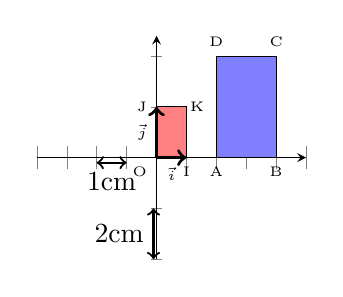
\begin{tikzpicture}
    \begin{axis}[
      width = 5cm,
      height = 3cm,
      xmax = 5,
      xmin = -4,
      ymin = -2,
      ymax = 2.4,
      yscale = 2,
      xscale = 1.,
      xtick distance = 1,
      ytick distance = 1,
      xticklabels = {},
      yticklabels = {},
      axis x line= center,
      axis y line= center        
      ]
      \addplot [domain=0:1, samples=20, fill=red!50!white] {1}
      \closedcycle;
      \addplot [->,very thick] coordinates {( 0,0)(1,0)};
      \addplot [->,very thick] coordinates {( 0,0)(0,1)};
      \node at (axis cs: 0,0) [below left] {\tiny O};
      \node at (axis cs: 1,0) [below] {\tiny I};
      \node at (axis cs: 0.8,1) [right] {\tiny K};
      \node at (axis cs: 0,1) [left] {\tiny J};
      \node at (axis cs: 0.5,0) [below] {$\scriptscriptstyle{\vec{i}}$};
      \node at (axis cs: 0,0.5) [left] {$\scriptscriptstyle{\vec{j}}$};
      \addplot [<->,thick] coordinates {(
        -2,-0.1)(-1,-0.1)};
      \addplot [<->,thick] coordinates {(
        -0.1,-2)(-0.1,-1)};
      \node at (axis cs: -1.5,-0.1) [below] {1cm};
      \node at (axis cs: -0.1,-1.5) [left] {2cm};

      \addplot [domain=2:4, samples=20, fill=blue!50!white] {2}
      \closedcycle;
      \node at (axis cs: 2,0) [below] {\tiny A};
      \node at (axis cs: 4,0) [below] {\tiny B};
      \node at (axis cs: 4,2) [above] {\tiny C};
      \node at (axis cs: 2,2) [above] {\tiny D};
    \end{axis}
  \end{tikzpicture}
\end{minipage}
\hfill
\begin{minipage}{0.45\linewidth}
  Dans cet exemple on a 1 \textbf{u.a} $= 1 \times 2 = 2cm^2$
  Ainsi on à l'aire du rectangle ABCD qui est:
  \[
    \mathcal{A}(ABCD) = 2u.x*2u.y = 4 \text{ \textbf{ua} } = 8 cm^2
  \]
  où u.x et u.y représente l'unité des abscisses et u.y l'unité des
  ordonnées. 
\end{minipage}

\subsubsection{Approche de la notion d'intégrale}

\begin{minipage}{0.45\linewidth}
\begin{center}
  \begin{tikzpicture}
    \begin{axis}[
      width = 8cm,
      height = 6cm,
      xmax = 5,
      xmin = -1,
      ymin = -1,
      ymax = 3,
      xtick distance = 1,
      ytick distance = 1,
      xticklabels = {},
      yticklabels = {},
      axis x line= center,
      axis y line= center        
      ]

      %\addplot[domain=1:1.9, samples=20, fill=orange!30!white] {-1/x + 2};

      \addplot[name path = g,domain=1:4, samples=20] {-1/x + 2};

      \addplot[domain=0:1.9] {-1/1.9+2};
      
      \addplot[domain=1.9:2.1,
      samples=50,fill=green!50!white, postaction={pattern=north east lines}]
      {-1/1.9 + 2}\closedcycle;

      \node at (axis cs: 0,0) [below left] {O};
      \addplot [->,very thick] coordinates {( 0,0)(1,0)};
      \addplot [->,very thick] coordinates {( 0,0)(0,1)};
      
            
      \node at (axis cs: 0.5,0) [below] {$\scriptscriptstyle{\vec{i}}$};
      \node at (axis cs: 0,0.5) [left]
      {$\scriptscriptstyle{\vec{j}}$};

      \path[name path=axis] (axis cs:1,0) -- (axis cs:4,0);
      
      \addplot [thick,fill=orange!30!white]
      fill between [ of=g and axis];

      \node at (axis cs: 0,{-1/1.9+2}) {$\bullet$};
      \node at (axis cs: 0,{-1/1.9+2}) [left] {\small f(x)};

      \addplot [<->] coordinates {(1.9,-0.1)(2.1,-0.1)};
      \node at (axis cs: 1.95,-0.1) [below] {\small h};

      \node at (axis cs: 4,0) [below] {\small b};
      \node at (axis cs: 1,0) [below] {\small a};
    \end{axis}
  \end{tikzpicture}
\end{center}
\end{minipage}
\begin{minipage}{0.45\linewidth}
  On appelle $\mathcal{A}$ l'aire de la surface orange situé sous la
  courbe et mesurée en unité d'aire.

  \vspace{1\baselineskip}
  
  L'aire du rectangle vert sur la figure est égale à $h \times
  f(x)$. On pourrait approcher l'aire de la surface orange en
  recouvrant celle-ci par des rectangles de ce type pour x variant de
  a à b et en sommant leurs aires. Plus h deviendra \og petit\fg{}
  plus la somme des aires des rectangles sera \og proche\fg{} de $\mathcal{A}$.
\end{minipage}

Si l'on exprime ça de manière \og plus mathématiques\fg{} on dira que
la somme des h*f(x) tend vers $\mathcal{A}$ lorsque h tend vers 0,
pour x allant de a à b.

Cette limite de somme est notée avec le symbole $\int$ qui se lit
intégrale. Les bornes de l'intervalle sont appelés bornes de
l'intégrale et notées :$\int_a^b$.

\subsection{Intégrale d'une fonction continue positive: }
\begin{mydef}
  On appelle \textbf{hypographe} d'une fonction f défini sur un
  intervalle I l'ensemble noté $hyp f$:
  \[
    hyp f = \{ (x,\alpha) \in I \times \R | ~f(x) \geq \alpha \}
  \]
\end{mydef}

Ainsi, pour une fonction f continue et positive sur un intervalle I=(a,b),
l'hypographe est la partie du plan délimitée par:
\begin{itemize}
\item la courbe représentative de f
\item l'axe des abscisses
\item la droite d'équation x = a
\item la droite d'équation x = b
\end{itemize}

\begin{mydef}
  Soient $a,b \in \R$ avec a<b. Soit $f:[a,b] \to \R$  une fonction
  positive et continue. On appelle intégrale de a à b et on note
  $\int_a^b f(t) dt$ la mesure de l'aire de l'hypographe de f défini
  ci-dessus. 
\end{mydef} 

\begin{Rem}
  \begin{enumerate}[label = (\alph*), leftmargin=2cm]
  \item a et b sont appelés bornes de l'intégrale.
  \item t est appelé la variable d'intégration qui est une variable
    muette. Elle peut donc être remplacé par n'importe quelle lettre
    et ne sert qu'à réaliser les calculs.
  \end{enumerate}
\end{Rem}

\exemple{}

\subsection{Intégrale d'une fonction continue négative: }
\begin{mydef}
  On appelle \textbf{épigraphe} d'une fonction f défini sur un
  intervalle I l'ensemble noté $epi f$:
  \[
    epi f = \{ (x,\alpha) \in I \times \R | ~f(x) \leq \alpha \}
  \]
\end{mydef}

Ainsi, pour une fonction f continue et négative sur un intervalle I=(a,b),
l'épigraphe est la partie du plan délimitée par:
\begin{itemize}
\item la courbe représentative de f
\item l'axe des abscisses
\item la droite d'équation x = a
\item la droite d'équation x = b
\end{itemize}

\begin{mydef}
  Soient $a,b \in \R$ avec a<b. Soit $f:[a,b] \to \R$  une fonction
  négative et continue. On appelle intégrale de a à b et on note
  $\int_a^b f(t) dt$ l'opposé de la mesure de l'aire de l'épigraphe de f défini
  ci-dessus. 
\end{mydef} 

\subsection{Intégrale d'une fonction continue}
\begin{mydef}
  Soient $a,b \in \R$ avec a<b. Soit $f:[a,b] \to \R$  une fonction
  continue. On appelle intégrale de a à b et on note
  $\int_a^b f(t) dt$ la différence entre:
  \begin{itemize}[label=$\bullet$, leftmargin=2cm]
  \item La mesure de l'aire de $f^+=max(0,f)$ et
  \item la mesure de l'aire de $f^-=max(-f,0)$
  \end{itemize}
\end{mydef}

\note Graphique
\section{Lien entre intégrale et primitives}
\begin{theo}
  Soit f une fonction continue sur un intervalle I. La fonction F
  définie sur I par $\int_a^x f(t) dt$ est l'unique primitive de la fonction
  f s'annulant en a. Si G est une primitive de f quelconque on a :
  \[
    \int_a^b f(t) dt = G(b) - G(a)
  \]
\end{theo}

\begin{Proof}
  \textbf{Cas monotone: f croissante}

  Calculons la limite du taux d'accroissement de F. On a :
  \[
    T_h(F) = \frac{F(x+h)-F(x)}{h} = \frac{\int_x^{x+h} f(t) dt}{h}
  \]

  Supposons (sans perte de généralité) que h>0. Ainsi on a $\cancel{h}
  \frac{f(x)}{\cancel{h}} \leq T_h(F) \leq \cancel h \frac{f(x+h)}{h}$
  car f est croissante. Puisque f est continue on a $\lim
  \limits_{h\to 0} f(x+h) = f(x)$ et donc d'après le théorème des
  gendarmes on a:
  \[
    \lim \limits_{h \to 0} T_h(F) = f(x)
  \]
  Et donc par définition du nombre dérivée, $F'(x) = f(x)$ (F(a) = 0 OK)

  De ce fait on a, $F(b) = \int_a^b f(t) dt$. Puisque $F(a) = 0$ on a
  aussi $F(b)-F(a) = \int_a^b f(t)dt$. Si G est une autre primitive de
  f, la formule est également vraie car $G(x) = F(x)+k$ pour tout x de
  I avec k constante réel.

  \textbf{Cas général}
  
  Utilisons la continuité de f. On se fixe $x \in I$. Puisque f est continue on a:
  \[
    \forall \varepsilon>0, ~ \exists \eta>0 ~\big( \forall t \in I,~ |x-t|<\eta
    \Rightarrow |f(x)-f(t)|<\varepsilon \big)
  \]

  Soit $\varepsilon >0$. Prenons h t.q. $|h|<=\frac{\eta}{2}$. On a donc
  \[
    f(x) - \varepsilon < f(t) < f(x) + \varepsilon ~ \forall t \in [x,x+h]
  \]

  Ainsi $f(x)-\epsilon < T_h(F) < f(x)+\varepsilon \Leftrightarrow
  |T_h(F) - f(x)| < \varepsilon $. Finalement on a montré:
  \[
    \forall \varepsilon > 0, ~ \exists \eta>0,~\big( \forall h ~ |h| < \eta
    \Rightarrow |T_h(F) - f(x)|<\varepsilon \big) 
  \]
  
\end{Proof}

%%% Local Variables:
%%% mode: latex
%%% TeX-master: "Experience_aleatoire"
%%% End:
